As illustrated by Figure \ref{fig:rectenna_circuit}, the rectifier consists of a single diode as the source of nonlinearity and a low-pass filter to store energy.

\begin{figure}
  \centering
    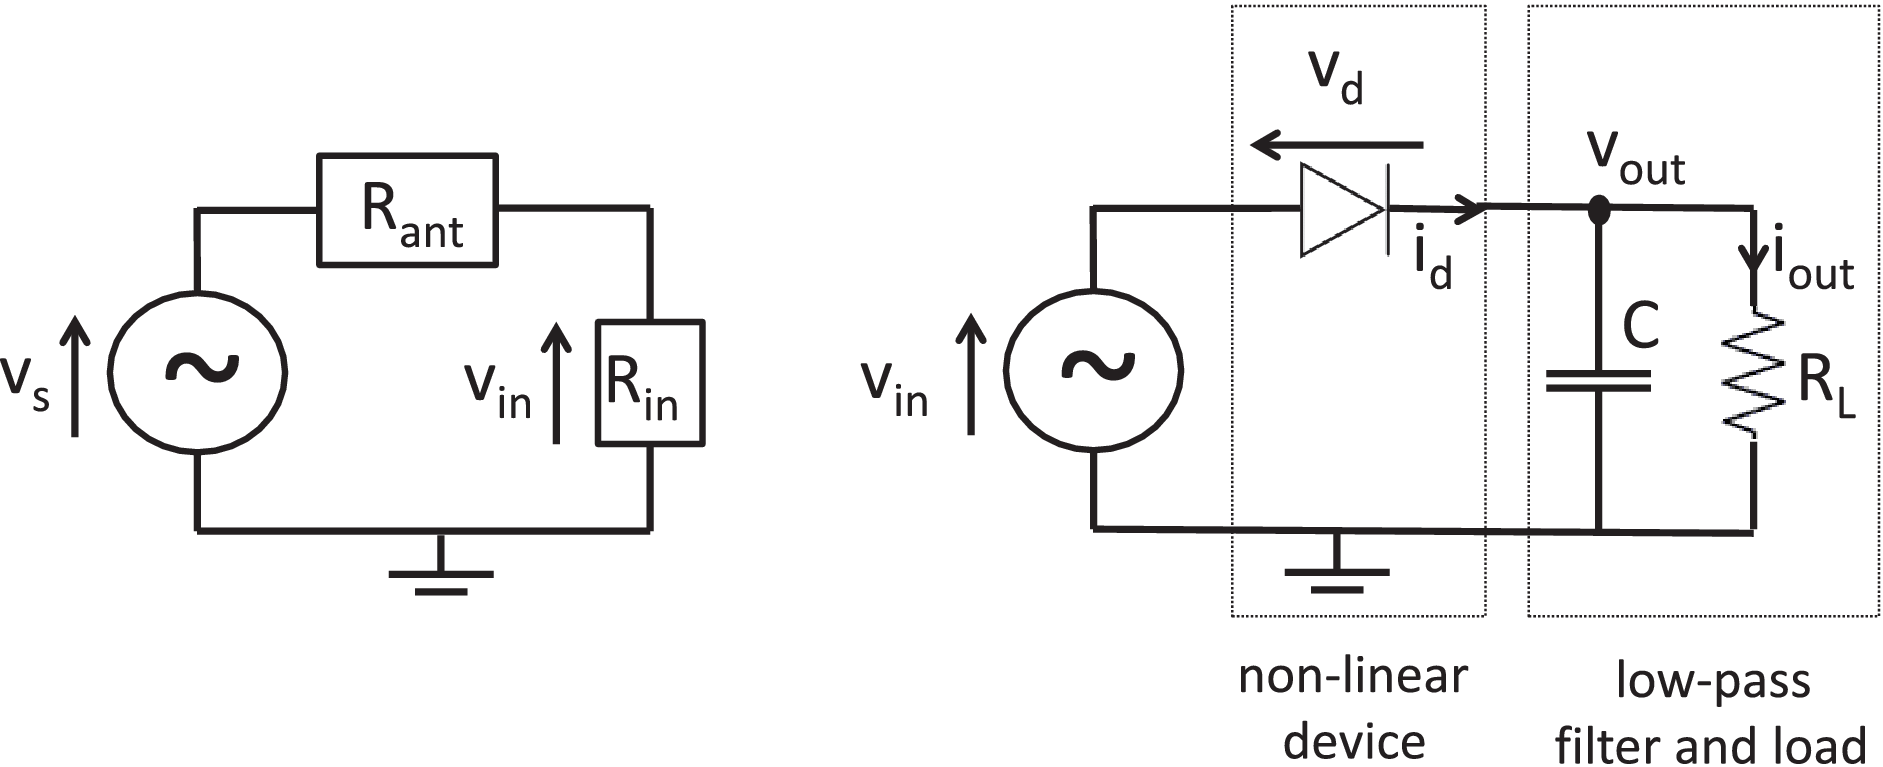
\includegraphics[width=\textwidth]{rectenna_circuit}
  \caption{Rectenna equivalent circuit (left) and a single diode rectifier (right) \cite{Clerckx2018a}}
  \label{fig:rectenna_circuit}
\end{figure}

Assume lossless, the equivalent circuit includes a voltage source ${v_{\text{s}}}(t)$ connected to a series antenna impedance ${Z_{{\text{ant}}}} = {R_{{\text{ant}}}} + j{X_{{\text{ant}}}}$ followed by a combined impedance of the rectifier and the matching network ${Z_{{\text{in}}}} = {R_{{\text{in}}}} + j{X_{{\text{in}}}}$. The perfect matching condition is

\begin{equation}\label{eqn:perfect_match}
  {R_{{\text{in}}}} = {R_{{\text{ant}}}},{X_{{\text{in}}}} =  - {X_{{\text{ant}}}}
\end{equation}

When equation \ref{eqn:perfect_match} is satisfied, the rectifier input voltage equals

\begin{equation}\label{eqn:rectifier_input_voltage}
  {v_{{\text{in}}}}(t) = {v_{\text{s}}}(t)/2 = y(t)\sqrt {{R_{{\text{in}}}}}
\end{equation}

where ${y(t)}$ is the received signal. Therefore, the input power to the rectifier writes

\begin{equation}\label{eqn:rectifier_input_power}
  P_{{\text{rf}}}^r = \mathbb{E}\left[ {y{{(t)}^2}} \right] = \mathbb{E}\left[ {{v_{{\text{in}}}}{{(t)}^2}} \right]/{R_{{\text{in}}}}
\end{equation}

It is also assumed that the noise is too small to be harvested.
